% Copyright Luke Olson 2009--2014
% This work is licensed under the Creative Commons
% Attribution-NonCommercial-NoDerivatives 4.0 International License. To view a
% copy of this license, visit http://creativecommons.org/licenses/by-nc-nd/4.0/.
%
\documentclass[10pt]{beamer}
%\documentclass[handout,10pt]{beamer}
%
\mode<presentation>
{
  \usetheme{Boadilla}
  \usecolortheme{luke}
  \usefonttheme[onlymath]{serif}
  \setbeamercovered{invisible}
  %\setbeamercovered{transparent}
}
\mode<handout>
{
  \usetheme{Boadilla}
  \usecolortheme{luke2}
  \usefonttheme[onlymath]{serif}
  \setbeamercovered{invisible}
  %\setbeamercovered{transparent}
}
\usepackage{pgf}
\usepackage{pxfonts}
\usepackage{eulervm}
\usepackage{listings}
%
%
%
\newcommand{\vb}{{\bf{b}}}
\newcommand{\ve}{{\bf{e}}}
\newcommand{\vg}{{\bf{g}}}
\newcommand{\vp}{{\bf{p}}}
\newcommand{\vr}{{\bf{r}}}
\newcommand{\vu}{{\bf{u}}}
\newcommand{\vx}{{\bf{x}}}
\newcommand{\vz}{{\bf{z}}}
\newcommand{\vA}{{\bf{A}}}
\newcommand{\vU}{{\bf{U}}}
\newcommand{\mO}{{\mathcal{O}}}
\newcommand{\mF}{{\mathcal{F}}}
\definecolor{mygray}{rgb}{0.95,0.95,0.95}
\lstset{
        language=matlab,
        numbers=left, numberstyle=\tiny, stepnumber=1, numbersep=5pt,
        basicstyle=\color{black}\ttfamily\small,
        commentstyle=\color{green}\ttfamily,
        keywordstyle=\color{blue}\ttfamily,
        stringstyle=\color{red}\ttfamily,
        showstringspaces=false,
        backgroundcolor=\color{mygray},
        breaklines,
}

\author{L. Olson}
\institute[UIUC]
{Department of Computer Science\\
University of Illinois at Urbana-Champaign\\
\vspace{0.5cm}
}
%%%%%%%%%%%%%%%%%%%%%%%%%%%%%%%%%%%%%%%%%%%%%%%%%%%%%%%%%%%%%%%%%%%%%%%%
%%%%%%%%%%%%%%%%%%%%%%%%%%%%%%%%%%%%%%%%%%%%%%%%%%%%%%%%%%%%%%%%%%%%%%%%
\title[CS 357]{Lecture 2}
\subtitle{Computational Experiments, Matlab, Randomness}
\date{August 27, 2009}

\begin{document}
% -------------------------------------------------
\begin{frame}
  \titlepage
\end{frame}
% -------------------------------------------------
\begin{frame}
\frametitle{What we'll do:}
\begin{itemize}
  \item get introduced to the basics of Matlab
  \item learn how to \emph{test} numerical methods, not just run them
  \item investigate ``randomness''
\end{itemize}
\end{frame}
% -------------------------------------------------
% -------------------------------------------------
\begin{frame}
\frametitle{Why this is important:}
\begin{itemize} 
  \item When developing code often a proof-of-concept is easier in a
higher-level environment
    \begin{itemize}
      \item Matlab or Octave (open source)
      \item Python + Numpy + Scipy front-end, C/C++ backend
      \item R (statistical)
      \item ...
    \end{itemize}
  \item When posed with a problem, we have a myriad of options (a.k.a. methods)
.  To choose the correct tools, we need to know how well it ``works''
    \begin{itemize}
      \item accuracy for the problem
      \item speed for the problem
      \item implementation ease
      \item memory footprint
    \end{itemize}
  \item Our testing and our methods often rely on ``randomness'' and the impact
of finite precision
    \begin{itemize}
      \item Random input
      \item Random perturbations
      \item Random sequences
    \end{itemize}
\end{itemize}
\end{frame}
% -------------------------------------------------
% -------------------------------------------------
\begin{frame}
\frametitle{What is MATLAB?}
\begin{itemize}
\item both a computing environment and a language
\item initially developed as an easy interface to LAPACK: Linear Algebra
Package (FORTRAN libraries)
\item {\bf MAT}rix {\bf LAB}oratory
\item Written in C.  For matrix computations, it calls C/Fortran libraries == Fast
\item Matlab + "Toolboxes"
  \begin{itemize}
  \item Symbolic Math Toolbox: mathematical manipulation of symbols
  \item Partial Differential Equation Toolbox: tools for solving PDEs in 2-D
  \item Statistics Toolbox: statistical data analysis
  \item Image processing toolbox: visualization and image analysis
  \item Bioinformatics toolbox: computational molecular biology
  \item Compiler: application development
  \item many many more.
  \end{itemize}
\item {\url{http://www.mathworks.com}}
\end{itemize}
\end{frame}
% -------------------------------------------------
% -------------------------------------------------
\begin{frame}
\frametitle{Why Matlab?}
The Good:
\begin{itemize}
\item Fast development times
\item no compiling, easy debugging
\item accessible syntax and language constructs
\item in-house graphics capabilities
\item tons of basic "libraries" or functions available
\item many more complicated "toolboxes" can be added
\end{itemize}
The Bad:
\begin{itemize}
\item small coding mistakes can result in slow code
\item loops are extremely computationally intensive
\item language is limited: no templates, classes etc.
\end{itemize}
The Ugly:
\begin{itemize}
\item proprietary (but the language format is open)
\item expensive (but free for UIUC students/faculty through webstore)
\item the open source substitute, Octave, is not fully compatible
\end{itemize}
\end{frame}
% -------------------------------------------------
% -------------------------------------------------
\begin{frame}[shrink]
\frametitle{Interpreter vs.~Scripts vs.~Functions}
\pgfimage[height=9cm]{figs/scriptvsfunc}
\end{frame}
% -------------------------------------------------
% -------------------------------------------------
\begin{frame}
\frametitle{Interpreter vs.~Scripts vs.~Function}
Interpreter:
\begin{itemize}
\item quick access
\item good for developing ideas
\item good for accessing data in the workspace
\item poor performance and editing/debugging capabilities
\end{itemize}
Script
\begin{itemize}
\item good test bed: all info in the workspace
\item fast, linear
\item poor profiling/optimization
\end{itemize}
Functions
\begin{itemize}
\item can be optimized and cached
\item don't fill up the workspace with memory that you have to manage,
but...
\item pass by value (ouch!)
\item reusable code
\end{itemize}
\end{frame}
% -------------------------------------------------
% -------------------------------------------------
\begin{frame}
\frametitle{Functions}
\begin{itemize}
  \item save in \emph{functionname}.m
  \item can have 0, n, or variable number of inputs
  \item can have 0, n, or variable number of outputs
  \item use {\texttt{return;}} to leave a function early
  \item use {\texttt{inline(...)}} to define without another file
  \item variables not "passed in" are \emph{local}: only available within
  the function scope
  \item use {\texttt{global}} \emph{varname;} to declare a variable that is
  visible through all functions
\end{itemize}
\end{frame}
% -------------------------------------------------
% -------------------------------------------------
\begin{frame}
\frametitle{More on Matlab...}
\begin{itemize}
\item new to Matlab: {\url{http://www.cse.uiuc.edu/heath/scicomp/software/matlab.html}}
\item free numerics book: {\url{http://www.mathworks.com/moler/index.html}}
\item TA tutorial tonight in DCL
\end{itemize}
\end{frame}
% -------------------------------------------------
% -------------------------------------------------
\begin{frame}
\frametitle{Last Time: Taylor Series}
\begin{itemize}
  \item How do we evaluate $f(x) = \frac{1}{1-x}$ computationally?
  \item Taylor Series Expansion:
\begin{equation*}
    f(x) = f(c) + (x-c) f'(c) + \frac{(x-c)^2}{2!} f''(c) + \dots +
\frac{(x-c)^n}{n!} f^{(n)}(\xi),
\end{equation*}
  \item Thus with c = 0
  \begin{equation*}
  \frac{1}{1-x} = 1 + x + x^2 + x^3 + \dots
\end{equation*}
  \item Second order approximation:
  \begin{equation*}
  \frac{1}{1-x} \approx 1 + x + x^2
\end{equation*}
\end{itemize}
\end{frame}
% -------------------------------------------------
% -------------------------------------------------
\begin{frame}
\frametitle{Taylor Errors}
\begin{itemize}
  \item How many terms do I need to make sure my error is less than
$2 \times 10^{-8}$ for $x=1/2$?
  \begin{equation*}
  \frac{1}{1-x} = 1 + x + x^2 + \dots + x^{n} + \sum_{k=n+1}^{\infty} x^k
  \end{equation*}
  \item so the error at $x=1/2$ is
  \begin{align*}
  e_{x=1/2} & = \sum_{k=n+1}^{\infty} \left(\frac{1}{2}\right)^k
            = \frac{(1/2)^{n+1}}{1-1/2}\\
            & = 2\cdot(1/2)^{n+1} < 2\times 10^{-8}\\
  \end{align*}
  \item then we need
    \begin{align*}
      n+1 & > \frac{-8}{\log_{10}(1/2)} \approx 26.6\quad\text{or}\\
      n &> 26
\end{align*}
\end{itemize}
\end{frame}
% -------------------------------------------------
\begin{frame}
\frametitle{Errors}
\begin{itemize}
  \item How do I classify my method?
  \item Goal: determine how the error $|f(x) - p_n(x)|$ behaves relative to $n$
(and $f$).
  \item Goal: determine how the cost of computing $p_n(x)$ behave relative to
$n$ (and $f$).
  \item for $f(x) = \frac{1}{1-x}$ we have
\[
  p_n = \sum_{k=0}^{n} x^k = 1 + x + x^2 + \dots
\]
  \item so
    \[
    e_n = |f(x) - p_n(x)|
\]
  \item Is $e_n \sim 1/n^{r}$?
  \item Is $e_n \sim 1/\sqrt{n}$?
  \item Is $e_n \sim 1/n!$?
\end{itemize}
\end{frame}
% -------------------------------------------------
%%%%%%%%%%%%%%%%%%%%%%%%%%%%%%%%%%%%%%%%%%%%%%%%%%%%%%%%%%%%%%%%%%%%%%%%
\begin{frame}
\frametitle{Big-O}
How to measure the impact of $n$ on algorithmic cost?
\begin{block}{$\mO(\cdot)$}
Let $g(n)$ be a function of $n$.  Then define
\begin{equation*}
  \mO(g(n)) = \{f(n)\,|\, \exists c,n_0>0 \,:\, 0\leq f(n)\leq cg(n),\, \forall
n\geq n_0\}
\end{equation*}

That is, $f(n)\in \mO(g(n))$ if there is a constant $c$ such that $0\leq f(n)
\leq cg(n)$ is satisfied.
\end{block}
\begin{itemize}
  \item assume non-negative functions (otherwise add $| \cdot |$) to the definitions
  \item $f(n)\in\mO(g(n))$ represents an asymptotic upper bound on $f(n)$ up to a constant
  \item example: $f(n) = 3\sqrt{n} + 2\log n + 8 n + 85 n^2 \in \mO(n^2)$
\end{itemize}
\end{frame}
%%%%%%%%%%%%%%%%%%%%%%%%%%%%%%%%%%%%%%%%%%%%%%%%%%%%%%%%%%%%%%%%%%%%%%%%
%%%%%%%%%%%%%%%%%%%%%%%%%%%%%%%%%%%%%%%%%%%%%%%%%%%%%%%%%%%%%%%%%%%%%%%%
\begin{frame}
\frametitle{Big-O (Omicron)}
\framesubtitle{asymptotic upper bound}
\begin{block}{$\mO(\cdot)$}
Let $g(n)$ be a function of $n$.  Then define
\begin{equation*}
  \mO(g(n)) = \{f(n)\,|\, \exists c,n_0>0 \,:\, 0\leq f(n)\leq cg(n),\, \forall
n\geq n_0\}
\end{equation*}

That is, $f(n)\in \mO(g(n))$ if there is a constant $c$ such that $0\leq f(n)
\leq cg(n)$ is satisfied.
\end{block}
\begin{center} 
  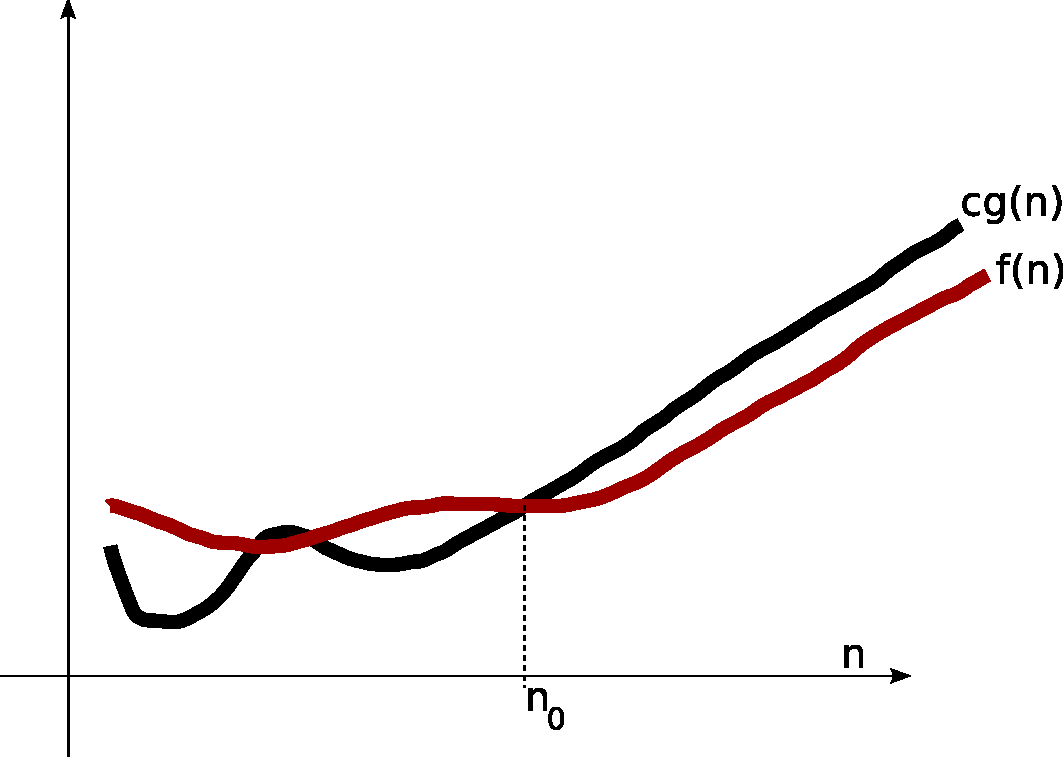
\includegraphics[height=4cm]{./figs/bigo_1}
\end{center}
\end{frame}
%%%%%%%%%%%%%%%%%%%%%%%%%%%%%%%%%%%%%%%%%%%%%%%%%%%%%%%%%%%%%%%%%%%%%%%%
%%%%%%%%%%%%%%%%%%%%%%%%%%%%%%%%%%%%%%%%%%%%%%%%%%%%%%%%%%%%%%%%%%%%%%%%
\begin{frame}
\frametitle{Big-Omega}
\framesubtitle{asymptotic lower bound}
\begin{block}{$\Omega(\cdot)$}
Let $g(n)$ be a function of $n$.  Then define
\begin{equation*}
  \Omega(g(n)) = \{f(n)\,|\, \exists c,n_0>0 \,:\, 0\leq cg(n) \leq f(n),\, \forall n\geq n_0\}
\end{equation*}

That is, $f(n)\in \Omega(g(n))$ if there is a constant $c$ such that $0\leq cg(n) \leq f(n)$ is satisfied.
\end{block}
\begin{center}
  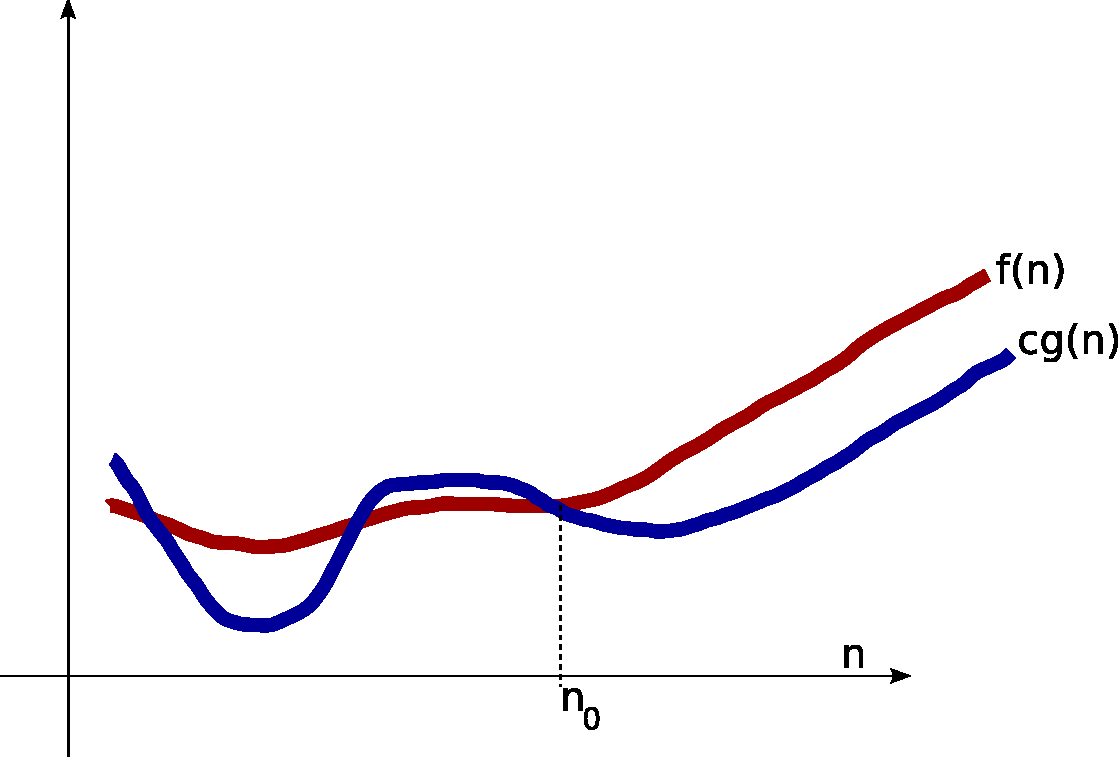
\includegraphics[height=4cm]{./figs/bigo_2}
\end{center}
\end{frame}
%%%%%%%%%%%%%%%%%%%%%%%%%%%%%%%%%%%%%%%%%%%%%%%%%%%%%%%%%%%%%%%%%%%%%%%%
%%%%%%%%%%%%%%%%%%%%%%%%%%%%%%%%%%%%%%%%%%%%%%%%%%%%%%%%%%%%%%%%%%%%%%%%
\begin{frame}
\frametitle{Big-Theta}
\framesubtitle{asymptotic tight bound}
\begin{block}{$\Theta(\cdot)$}
Let $g(n)$ be a function of $n$.  Then define
\begin{equation*}
  \Theta(g(n)) = \{f(n)\,|\, \exists c_1,c_2,n_0>0 \,:\, 0\leq c_1g(n) \leq
f(n)\leq c_2 g(n),\, \forall
n\geq n_0\}
\end{equation*}

Equivalently, $\Theta(g(n)) = \mO(g(n)) \cap \Omega(g(n))$.
\end{block}

\begin{center}
  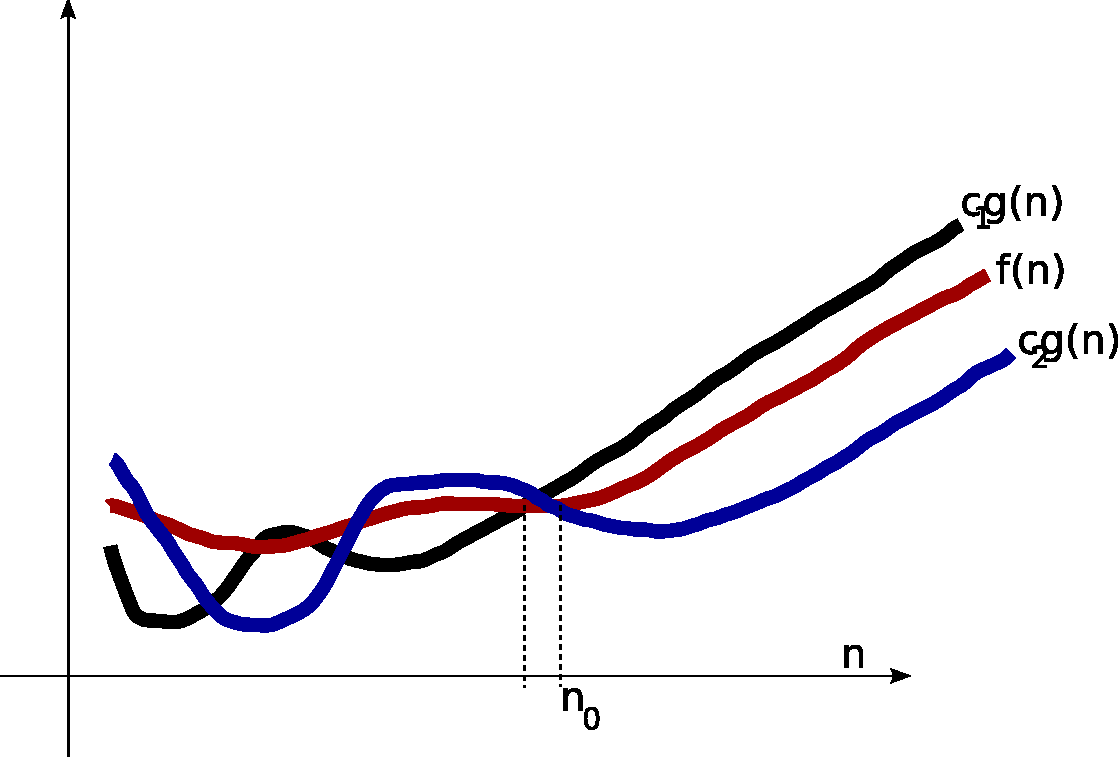
\includegraphics[height=4cm]{./figs/bigo_3}
\end{center}
\end{frame}
%%%%%%%%%%%%%%%%%%%%%%%%%%%%%%%%%%%%%%%%%%%%%%%%%%%%%%%%%%%%%%%%%%%%%%%
% -------------------------------------------------
\begin{frame}
\frametitle{Algebraic Convergence (J. P. Boyd)}
\begin{block}{Definition}
The {\underline {Algebraic Index of Convergence}} $\alpha$ is the largest number for which
\[
	\lim_{n\rightarrow\infty} |a_{n}| n^{\alpha} < \infty
	\]
	where $a_{n}$ are the coefficients in the sequence.  Alternatively, $\alpha$ is the algebraic index if
	\[
	a_{n} \sim \mO(1/n^{\alpha})
	\]
\end{block}
\end{frame}
% -------------------------------------------------
% -------------------------------------------------
\begin{frame}
\frametitle{Exponential Convergence (J. P. Boyd)}
\begin{block}{Definition}
If the algebraic index $\alpha$ is unbounded (i.e. $a_{n}$ decrease faster than
$1/n^{\alpha}$ for any finite $\alpha$), then the sequence converges {\underline{exponentially}} (a.k.a. {\underline{spectrally}}).
\bigskip

Alternatively, the sequence converges exponentially if for constants $q$ and $\beta$
	\[
	a_{n} \sim \mO(e^{-q n^{\beta}})
	\]
	where $\beta$ is the {\underline{exponential index of convergence}} and
	\[
	\beta = \lim_{n\rightarrow\infty}\frac{\log | \log(|a_{n}|) |}{\log(n)}
	\]
\end{block}
\end{frame}
% -------------------------------------------------
\begin{frame}
\frametitle{Rates of Exponential Convergence (J. P. Boyd)}
\begin{block}{Definition}
A sequence $a_{n}$ has {\underline{supergeometric}, \underline{geometric}, or \underline{subgeometric}} if
\[
\lim_{n\rightarrow\infty} \log(|a_{n}|)/n =
\begin{cases}
\infty, & \textnormal{supergeometric}\\
contant, & \textnormal{geometric}\\
0, & \textnormal{subgeometric}\\
\end{cases}
\]
\bigskip

or, alternatively,
\begin{align*}
a_{n} & \sim \mO(e^{-(n/j)\log(n)}): \,\,\textnormal{supergeometric} \\
a_{n} & \sim \mO(e^{-qn}): \,\,\textnormal{geometric} \\
\beta & < 1: \,\,\textnormal{subgeometric}\\
\end{align*}
\end{block}
\end{frame}
%--------
\begin{frame}
\frametitle{Asymptotic Rate of Geometric Convergence (J. P. Boyd)}
\begin{block}{definition}
If a sequence $a_{n}$ has geometric convergence ($\beta=1$) so that 
\[
a_{n} \sim \mO(e^{-n\mu})
\]
then the {\underline{asymptotic rate of geometric convergence}} is $\mu$.  Alternatively,
\[
\mu = \lim_{n\rightarrow\infty} \{ -\log |a_{n}|/n\}
\]
\end{block}
\end{frame}
%----------
\begin{frame}
\includegraphics[width=10cm]{./figs/conv1}
\end{frame}
\begin{frame}
\includegraphics[width=10cm]{./figs/conv2}
\end{frame}
\begin{frame}
\includegraphics[width=10cm]{./figs/conv3}
\end{frame}
\begin{frame}
\frametitle{But Taylor Series Approximations have many terms...}
  \begin{itemize}
  \item For example, how do we evaluate
  \begin{equation*}
  f(x) = 5x^3 + 3x^2 + 10 x + 8
\end{equation*}
at the point $1/3$?
  
  \item This would require 6 multiplications and 3 additions.
  \item If we regroup as
  \begin{equation*}
    f(x) = 8 + x(10 + x(3 + x(5)))
\end{equation*}
        then we have 3 multiplications and 3 additions.
  \item This is Nested Multiplication or Synthetic Division or Horner's
Method
\end{itemize}
\end{frame}
% -------------------------------------------------
% -------------------------------------------------
\begin{frame}[fragile]
\frametitle{Nested Multiplication}
  \begin{itemize}
    \item To evaluate
      \begin{equation*}
        f(x) = a_0 + a_1x + a_2 x^2 + \dots + a_n x^n
\end{equation*}
rewrite as
      \begin{equation*}
        f(x) = a_0 + x(a_1 + x(a_2 + \dots + x(a_n))\dots)
\end{equation*}
\end{itemize}
\begin{lstlisting}[mathescape,caption=nested mult]
$p=a_n$
for $i = n-1$ to 0 step -1
  $p = a_i + xp$
end
\end{lstlisting}
\end{frame}
% -------------------------------------------------
\begin{frame}
\frametitle{Randomness}
\framesubtitle{From M. Heath, \emph{Scientific Computing, 2nd ed.}, CS450}
\begin{itemize}
    \item Randomness $\approx$ unpredictability
    \item One view: a sequence is random if it has no shorter description
    \item Physical processes, such as flipping a coin or tossing dice, are
deterministic with enough information about the governing equations and initial
conditions.
    \item But even for deterministic systems, sensitivity to the initial
conditions can render the behavior practically unpredictable.
    \item we need random simulation methods
\end{itemize}
\bigskip

\url{http://dilbert.com/strips/comic/2001-10-25/}

\url{http://www.xkcd.com/221/}

\texttt{drunk.m}
\end{frame}
\begin{frame}
\frametitle{Randomness is easy, right?}
\begin{itemize}
\item 
In May, 2008, Debian announced a vulnerability with OpenSSL: the OpenSSL pseudo-random number generator
	\begin{itemize}
		\item the seeding process was compromised (2 years)
		\item only 32,767 possible keys
		\item seeding based on process ID (this is not entropy!)
		\item all SSL and SSH keys from 9/2006 - 5/2008 regenerated
		\item all certificates recertified
	\end{itemize}
	
\item Cryptographically secure pseudorandom number generator (CSPRNG) are necessary for some apps
\item Other apps rely less on true randomness
\end{itemize}
\end{frame}
\begin{frame}[fragile]
\frametitle{Repeatability}
\framesubtitle{From M. Heath, \emph{Scientific Computing, 2nd ed.}, CS450}
\begin{itemize}
    \item With unpredictability, true randomness is not repeatable
    \item ...but lack of repeatability makes testing/debugging difficult
    \item So we want repeatability, but also independence of the trials
\end{itemize}
\bigskip

\begin{lstlisting}
>> rand('seed',1234)  
>> rand(10,1)      
\end{lstlisting}

\end{frame}
\begin{frame}
\frametitle{Pseudorandom Numbers}
\framesubtitle{From M. Heath, \emph{Scientific Computing, 2nd ed.}, CS450}
\begin{alertblock}{}
    Computer algorithms for random number generations are deterministic
\end{alertblock}
\begin{itemize}
    \item ...but may have long periodicity (a long time until an apparent 
      pattern emerges)
    \item These sequences are labeled \emph{pseudorandom}
    \item Pseudorandom sequences are predictable and reproducible (this is
mostly good)
\end{itemize}
\end{frame}
\begin{frame}
\frametitle{Random Number Generators}
\framesubtitle{From M. Heath, \emph{Scientific Computing, 2nd ed.}, CS450}
Properties of a good random number generator:
\begin{description}
    \item[Random pattern:]  passes statistical tests of randomness
    \item[Long period:] long time before repeating
    \item[Efficiency:] executes rapidly and with low storage
    \item[Repeatability:] same sequence is generated using same initial states
    \item[Portability:] same sequences are generated on different architectures
\end{description}
\end{frame}
\begin{frame}
\frametitle{Random Number Generators}
\framesubtitle{From M. Heath, \emph{Scientific Computing, 2nd ed.}, CS450}
\begin{itemize}
    \item Early attempts relied on complexity to ensure randomness
    \item ``midsquare'' method: square each member of a sequence and take the
middle portion of the results as the next member of the sequence
    \item ...simple methods with a statistical basis are preferable
\end{itemize}
\end{frame}
\begin{frame}
\frametitle{Linear Congruential Generators}
\framesubtitle{From M. Heath, \emph{Scientific Computing, 2nd ed.}, CS450}
\begin{itemize}
    \item Congruential random number generators are of the form:
\[
x_k = (a x_{k-1} + c)\, (\mod M)
\]
where $a$ and $c$ are integers given as input.
    \item $x_0$ is called the \emph{seed}
    \item Integer $M$ is the largest integer representable (e.g. $2^{31} -1$)
    \item Quality depends on $a$ and $c$.  The period will be at most $M$.
\end{itemize}
\begin{example}
Let $a=13$, $c=0$, $m=31$, and $x_0=1$.
\[
1,\, 13,\, 14,\, 27,\, 10,\, 6,\, \dots
\]
This is a permutation of integers from $1,\dots,30$, so the period is $m-1$.
\end{example}
\bigskip

\texttt{randgui('rand')}

\texttt{randgui('randssp')}
\end{frame}
\begin{frame}
\frametitle{History} 
\framesubtitle{From C. Moler, emph{NCM}}
\begin{itemize}
    \item IBM used Scientific Subroutine Package (SSP) in the 1960's the
mainframes.
    \item Their random generator, $\texttt{rnd}$ used $a=65539$, $c=0$, and
$m=2^{31}$.
    \item arithmetic mod $2^{31}$ is done quickly with 32 bit words.
    \item multiplication can be done quickly with $a=2^{16}+3$ with a shift and
short add.
    \item Notice (mod $m$):
\[
    x_{k+2} = 6x_{k+1} - 9 x_{k}
\]
...strong correlation among three successive integers
\end{itemize}
\end{frame}
\begin{frame}
\frametitle{History} 
\framesubtitle{From C. Moler, \emph{NCM}}
\begin{itemize}
    \item Matlab used $a = 7^5$, $c=0$, and $m=2^{31}-1$ for a while
    \item period is $m-1$.
    \item this is no longer sufficient
\end{itemize}
\bigskip

\texttt{randgui('randssp')}
\end{frame}
\begin{frame}[fragile]
\frametitle{what's used?}
Two popular methods:

1. Method of Marsaglia (period $\approx 2^{1430}$).
\begin{lstlisting}[mathescape]
Initialize $x_0,\dots, x_3$ and $c$ to random values given a seed

Let $s=2111111111 x_{n-4} + 1492 x_{n-3} 1776 x_{n-2} + 5115 x_{n-1} + c$

Compute $x_n= s \mod 2^{32}$

$c = floor(s/2^{32})$
\end{lstlisting}
\bigskip

2. \emph{rand()} in Unix uses $a=1103515245$, $c=12345$, $m=2^{31}$.
\bigskip

\begin{alertblock}{}
    Even the Marsaglia method produces points in $n-D$ on only a small number of
hyperplanes.
\end{alertblock}
\begin{alertblock}{}
    In general, the digits in random numbers are not themselves random...some
patterns reoccur much more often.
\end{alertblock}
\end{frame}
\begin{frame}
\frametitle{Linear Congruential Generators}
\framesubtitle{From M. Heath, \emph{Scientific Computing, 2nd ed.}, CS450}
\begin{itemize}
    \item sensitive to $a$ and $c$
    \item be careful with supplied random functions on your system
    \item period is $M$
    \item standard division is necessary if generating floating points in
$[0,1)$.
\end{itemize}
\bigskip

\url{http://www.cse.uiuc.edu/iem/random/pairplot/}
\end{frame}
\begin{frame}
\frametitle{Fibonacci}
\framesubtitle{From M. Heath, \emph{Scientific Computing, 2nd ed.}, CS450}
\begin{itemize}
    \item produce floating-point random numbers directly using differences,
sums, or products.
    \item Typical subtractive generator:
\[
x_k = x_{k-17} - x_{5}
\]
with ``lags'' of 17 and 5.
    \item Lags much be chosen very carefully
    \item negative results need fixing
    \item more storage needed than congruential generators
    \item no division needed
    \item very very good statistical properties
    \item long periods since repetition does not imply a period
\end{itemize}
\end{frame}
\begin{frame}
\frametitle{Sampling over intervals}
\framesubtitle{From M. Heath, \emph{Scientific Computing, 2nd ed.}, CS450}
    If we need a uniform distribution over $[a,b)$, then we modify $x_k$ on
$[0,1)$ by
\[
(b-a)x_k + a
\]
\end{frame}
\begin{frame}
\frametitle{Non-uniform distributions}
\framesubtitle{From M. Heath, \emph{Scientific Computing, 2nd ed.}, CS450}
\begin{itemize}
    \item sampling nonuniform distributions is much more difficult
    \item if the cumulative distribution function is invertible, then we can
generate the non-uniform sample from the uniform:
\[
f(t) = \lambda e^{-\lambda t},\quad t>0
\]
thus
\[
y_k = -\log(1-x_k)/\lambda
\]
where $x_k$ is uniform in $[0,1)$.
    \item ...not so easy in general
\end{itemize}
\end{frame}
\begin{frame}
\frametitle{Quasi-Random Sequences}
\framesubtitle{From M. Heath, \emph{Scientific Computing, 2nd ed.}, CS450}
\begin{itemize}
    \item For some applications, reasonable uniform coverage of the sample is
more important than the ``randomness''
    \item True random samples often exhibit clumping
    \item Perfectly uniform samples uses a uniform grid, but does not scale well
at high dimensions
    \item quasi-random sequences attempt randomness while maintaining coverage
\end{itemize}
\end{frame}
\begin{frame}
\frametitle{Quasi-Random Sequences}
\framesubtitle{From M. Heath, \emph{Scientific Computing, 2nd ed.}, CS450}
\begin{itemize}
    \item quasi random sequences are not random, but give random appearance
    \item by design, the points avoid each other, resulting in no clumping
\end{itemize}
\bigskip

\url{http://www.cse.uiuc.edu/iem/random/quasirnd/}
\end{frame}
\end{document}
